%% Manuscript prepared with the Elsevier CAS template (cas-sc.cls).
%% Compile: pdflatex manuscript-cas -> bibtex manuscript-cas -> pdflatex x2
\documentclass[a4paper,fleqn]{cas-sc}
%% No 'longnamesfirst': the first citation of a reference would otherwise expand
%% to the full author list (e.g. a 40-author consensus statement inline).
\usepackage[authoryear]{natbib}
\usepackage[utf8]{inputenc}
\usepackage{graphicx}
\usepackage{booktabs}
\DeclareUnicodeCharacter{03C1}{$\rho$}
\DeclareUnicodeCharacter{00B1}{$\pm$}
\DeclareUnicodeCharacter{00D7}{$\times$}
\DeclareUnicodeCharacter{2265}{$\geq$}
\DeclareUnicodeCharacter{2264}{$\leq$}
\DeclareUnicodeCharacter{2212}{$-$}
\DeclareUnicodeCharacter{00B9}{\textsuperscript{1}}
\DeclareUnicodeCharacter{00B2}{\textsuperscript{2}}
\DeclareUnicodeCharacter{00B3}{\textsuperscript{3}}
\DeclareUnicodeCharacter{2013}{--}
\DeclareUnicodeCharacter{2014}{---}
\DeclareUnicodeCharacter{2192}{$\rightarrow$}
\DeclareUnicodeCharacter{2248}{$\approx$}
\DeclareUnicodeCharacter{2019}{'}
\DeclareUnicodeCharacter{2020}{\textdagger{}}

\begin{document}
%% Required by the CAS bundle (cf. cas-sc-sample.tex): suppress hyperref bookmark
%% writing, which otherwise aborts the run with "\@@BOOKMARK" scan errors.
\let\WriteBookmarks\relax
\def\floatpagepagefraction{1}
\def\textpagefraction{.001}
\shorttitle{Cross-cohort reproducibility benchmark}
\shortauthors{WANG and LI}

\title[mode=title]{Cross-cohort reproducibility of CT-based lung cancer survival prediction:
ComBat corrects feature-space orientation but not discrimination}

\author[1]{Jiuyang WANG}
\fnmark[1]
\credit{Data curation, Formal analysis, Software, Writing -- original draft, Writing -- review and editing}

\author[1]{Yong LI}
\cormark[1]
\ead{liyongcsco@email.ncu.edu.cn}
\credit{Conceptualization, Methodology, Supervision, Funding acquisition, Writing -- review and editing}
\affiliation[1]{organization={Department of Oncology, The First Affiliated Hospital of Nanchang University},
            city={Nanchang},
            state={Jiangxi},
            country={China}}
\cortext[1]{Corresponding author}
\fntext[1]{ORCID: 0009-0007-0788-977X}

\begin{abstract}
Cross-cohort transport of CT-based survival models in non-small cell lung cancer is widely attributed to batch effects, and correction with ComBat is commonly assumed to restore performance. Across five public CT collections (781 imaging entries; 741 distinct original patient identifiers; 633 with survival data), we held feature extraction and model class fixed and evaluated two deployment scenarios. In the inductive scenario, all preprocessing was fitted in LUNG1 (n = 422) and applied to NSCLC-Radiogenomics (n = 211) without ComBat; the joint-model target-cohort C-index was 0.458. In the transductive scenario, imputation and ComBat were fitted on the combined 633-patient feature set using no target-cohort outcome labels; the corresponding C-index was 0.509. The latter setting requires unlabeled target-domain imaging and is therefore an external evaluation under target-domain adaptation, not strict external validation. ComBat reduced the mean absolute standardised difference between cohorts from 0.755 to 0.012, with no feature exceeding |d| = 0.8 after correction, and changed the target-cohort calibration slope from $-$0.327 to +0.815. Supplementary L2 patient-level bootstrap internal evaluation yielded a joint-model OOB C-index of 0.571 (95\% bootstrap percentile interval 0.523--0.615; 1,000 resamples), rather than an uncertainty estimate for the primary L1 models. Both scenarios failed to raise target-cohort discrimination above chance-level confidence bounds. Target-cohort recalibration was an apparent post hoc fit; it changed absolute-risk diagnostics but not C-index. The overlap between the ten most important components across cohorts was 10\%, and stability-selected subsets showed no consistent advantage over random subsets. Cross-cohort reproducibility therefore comprises orthogonal layers --- feature-space orientation, baseline hazard and discrimination --- that require separate reporting; a corrected feature distribution does not by itself imply a transportable model.
\end{abstract}

\begin{highlights}
\item ComBat removed cross-cohort feature shift but did not improve discrimination.
\item External C-index stayed at 0.507 (95\% CI 0.431--0.580) after batch correction.
\item Recalibration cut Brier scores by 40--52\% without changing the C-index.
\item Feature--outcome associations differed between cohorts (top-10 overlap 10\%).
\item Cross-cohort reproducibility comprises orthogonal layers needing separate reporting.
\end{highlights}

\begin{keywords}
Cross-cohort reproducibility \sep Radiomics \sep Batch effect correction \sep Survival prediction \sep External validation \sep Calibration \sep Lung cancer
\end{keywords}

\maketitle

\begin{figure}[htbp]
\centering

\includegraphics[width=\textwidth]{figures/Fig1.pdf}
\caption{\textbf{Study flow and cohort composition.} Five publicly available collections from The Cancer Imaging Archive (TCIA) contributed 781 imaging entries. Deduplication by original patient identifier yielded 741 distinct original IDs; this is not a confirmed biological unique-patient count. A further 24 LungCT-Diagnosis cases share a 30-digit StudyInstanceUID suffix with LUAD-CT-Survival/QIN-LUNG-CT cases. If these candidate links are treated as shared patients, the sensitivity count is 717. LUNG1 and NSCLC-Radiogenomics share no patients by patient identifier or full StudyInstanceUID. The OS analysis included 633 patients: NSCLC-Radiomics (LUNG1, n = 422) and NSCLC-Radiogenomics (n = 211). Because the historical ComBat fit used features from both cohorts, the latter is a target-cohort evaluation after cohort-level feature adaptation, not a validation untouched by target features. LungCT-Diagnosis (n = 61), QIN-LUNG-CT (n = 47), and LUAD-CT-Survival (n = 40; 20 long, 20 short) were not used to fit the OS model; LUAD-CT-Survival was used only for a separate diagnostic binary-endpoint analysis. Grey boxes show the imaging-entry, patient-ID, and OS-analysis counts. Panel letter a is shown in bold lowercase. TCIA, The Cancer Imaging Archive.}
\label{fig:1}
\end{figure}

\begin{figure}[htbp]
\centering

\includegraphics[width=\textwidth]{figures/Fig2.pdf}
\caption{\textbf{Feature distributions before and after ComBat correction.} Principal component analysis (PCA) projections of image-derived features in the two survival cohorts before and after ComBat correction. (a) Radiomic features (107 per patient) before correction. (b) Radiomic features after correction. (c) InceptionV3 embeddings (2048 per patient) before correction. (d) Embeddings after correction. Each point is one patient (LUNG1, n = 422, circles; NSCLC-Radiogenomics, n = 211, triangles); s = 12, alpha = 0.6, no marker edges. Features were median-imputed and standardised on the combined cohort before PCA; axes are the first two principal components, and the x and y ranges are shared between a and b and between c and d so that panels are directly comparable. Before correction the two cohorts occupied separated regions of feature space; after correction the projections overlapped. Corresponding summary statistics: mean absolute standardised difference 0.755 $\rightarrow$ 0.012 for radiomic features and 0.647 $\rightarrow$ 0.014 for embeddings; the proportion of features exceeding |d| = 0.8 fell from 47\% to 0\% (radiomics) and from 32\% to 0\% (embeddings). PCA, principal component analysis.}
\label{fig:2}
\end{figure}

\begin{figure}[htbp]
\centering

\includegraphics[width=\textwidth]{figures/Fig3.pdf}
\caption{\textbf{Calibration of the joint model in external and internal evaluation.} Calibration of the joint (clinical + radiomic + embedding) Cox model at 365, 730 and 1095 days. Rows: (a--c) external cohort (NSCLC-Radiogenomics, n = 211) with the original model; (d--f) external cohort after linear recalibration fitted on the external cohort, with the original predictions overlaid as open circles; (g--i) internal out-of-fold predictions in LUNG1 (n = 422) from five-fold cross-validation. Within each panel, patients were divided into four risk quartile groups; each point is the group-mean predicted survival plotted against Kaplan-Meier observed survival at that time point. The black dashed line is the identity (ideal) line. All panels share 0--1 axes. Recalibration moved the external calibration points onto the identity line and reduced the Brier score by 40--52\% (365 days: 0.1468 $\rightarrow$ 0.0884; 730 days: 0.2889 $\rightarrow$ 0.1380; 1095 days: 0.2801 $\rightarrow$ 0.1608) without changing the C-index. Recalibration was applied as a post hoc analysis of failure structure and is not proposed as a prospectively applicable correction. Panel letters a--i are shown in bold lowercase.}
\label{fig:3}
\end{figure}

\begin{figure}[htbp]
\centering

\includegraphics[width=\textwidth]{figures/Fig4.pdf}
\caption{\textbf{IPCW decision curves for the deep and joint models.}  Net benefit is shown at 365, 730 and 1095 days. Absolute event probabilities, \textbackslash{}(1-S(t\textbackslash{}mid x)\textbackslash{}), were derived from the Cox survival function and evaluated with fixed-horizon inverse-probability-of-censoring weights. Treat-all (dashed black) and treat-none (grey solid) are reference strategies. Shaded bands are 95\% percentile intervals from 2,000 patient bootstrap resamples of the evaluation set with LUNG1-fitted models held fixed; they quantify conditional evaluation-sample uncertainty. Rows show target-cohort evaluation under the transductive scenario (top), target-cohort evaluation under the inductive scenario (middle), and internal LUNG1 out-of-fold evaluation (bottom). The y-axis display range is $-$0.20 to 0.60; the complete Treat-all values, including values below the displayed range at high thresholds, are in Table DCA\_results.csv. The transductive scenario uses unlabeled target-cohort feature statistics for imputation and ComBat and is therefore not strict external validation. DCA, decision curve analysis; IPCW, inverse probability of censoring weighting.}
\label{fig:4}
\end{figure}

\begin{figure}[htbp]
\centering

\includegraphics[width=\textwidth]{figures/Fig5.pdf}
\caption{\textbf{Cross-cohort agreement of fitted Cox coefficients.} (a) Coefficients of the 89 components of the joint model fitted separately in LUNG1 (n = 422) and NSCLC-Radiogenomics (n = 211); each point is one component. Orange squares (s = 28) indicate the union of components among the ten largest absolute coefficients in each cohort (19 components); grey circles (s = 12) indicate the remaining components. The black dashed line is the identity line and the thin grey lines mark zero. (b) The ten components with the largest absolute LUNG1 coefficient, shown as paired bars giving their coefficient in LUNG1 (blue, solid) and the corresponding coefficient in NSCLC-Radiogenomics (green, hatched). The inset reports descriptive Spearman rank correlation between the coefficient vectors ($\rho$ = 0.223) and top-10 overlap (1/10, 10\%). No inferential p value is shown because the fitted components are not independent sampling units. Marker shape and bar hatching provide redundant grayscale cues. Coefficients were fitted with the same model specification and feature basis in both cohorts.}
\label{fig:5}
\end{figure}

\begin{figure}[htbp]
\centering
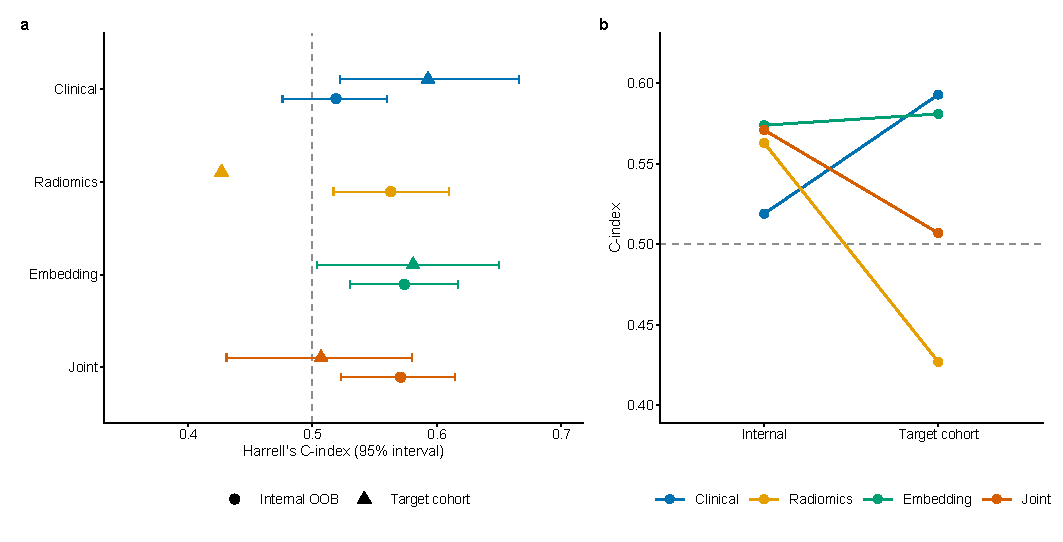
\includegraphics[width=\textwidth]{figures/Fig6.pdf}
\caption{\textbf{Internal-to-target-cohort discrimination by model.} (a) Harrell's C-index for the clinical, radiomic, embedding and joint models. Circles show supplementary internal out-of-bag estimates from the L2 patient-level bootstrap; triangles show target-cohort estimates from the primary L1 models. Horizontal bars are 95\% percentile intervals where available; no interval was computed for the radiomic target-cohort estimate. The dashed line marks chance-level discrimination (0.5). (b) Paired internal and target-cohort point estimates. Lines connect estimates for visual comparison only because the internal and target-cohort estimates use different penalties and resampling procedures and therefore do not define a matched transport-loss estimator.}
\label{fig:6}
\end{figure}

\begin{figure}[htbp]
\centering
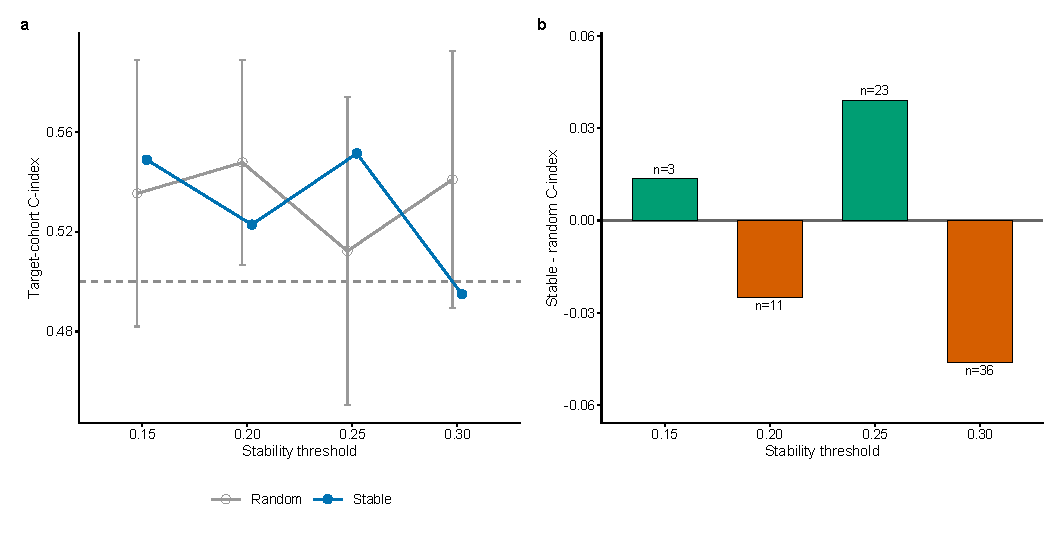
\includegraphics[width=\textwidth]{figures/Fig7.pdf}
\caption{\textbf{Stability-selected components do not consistently outperform size-matched random subsets.} (a) Target-cohort C-index for components retained at four coefficient-stability thresholds (blue) and the mean of size-matched random subsets (grey); error bars show the standard deviation across random subsets. The dashed line marks 0.5. (b) Difference between the stability-selected subset and the random-subset mean. Labels give the number of retained components. Positive and negative differences are shown in Okabe-Ito green and vermillion, respectively. All standardised differences from the random-subset distribution had |z| < 1; no inferential significance is claimed.}
\label{fig:7}
\end{figure}

\section{Introduction}

Quantitative analysis of pre-treatment computed tomography (CT) has been proposed as a source of prognostic information complementary to clinical staging in non-small cell lung cancer (NSCLC) \citep{aerts2014}. CT radiomic and deep-learning models have been evaluated for overall-survival prediction, including multi-cohort external evaluation \citep{amini2022,hosny2018}. Reviews and reporting guidance describe the expanding use of radiomics across imaging tasks while emphasising reproducibility and clinical-translation requirements \citep{mayerhoefer2020,vantimmeren2020,lambin2025}. External performance can decline materially relative to development-cohort estimates \citep{hosny2018,jha2023}, consistent with broader evidence that predictive systems can be fragile across sites \citep{zech2018,wynants2020}. Because cohorts differ in scanner, acquisition protocol, reconstruction kernel, and patient mix, distributional shift in the extracted features is a plausible contributor, and batch correction is a common response. Whether correction of marginal feature distributions restores outcome prediction remains an empirical question.

ComBat estimates and removes site-specific additive and multiplicative effects; it was introduced for microarray data \citep{johnson2007} and later adapted to multi-site imaging \citep{fortin2018}, including CT radiomics \citep{daano2020,mahon2020,bertolini2022,horng2022,cromb2020}. In radiomics, its success is commonly assessed with distributional diagnostics---the standardised mean difference between cohorts, visual overlap of principal components, or the proportion of features with a large effect size. These diagnostics describe the input features rather than the prediction task. A recent multimodal survival study illustrates single-cohort development with internal evaluation \citep{sahin2026}, whereas other studies compare feature-selection, modelling, harmonisation, or dataset strategies across specific settings \citep{amini2022,ge2023,le2023,chen2022,wang2022,wang2022b}. A meta-analysis in the adjacent task of pathological-response prediction reported high summary discrimination together with between-study heterogeneity \citep{jiang2026}. These studies do not establish whether correcting marginal feature shift is sufficient to restore survival-model transport. It therefore remains unclear whether a model that fails across cohorts does so because of correctable feature shift, because of an unfavourable baseline hazard in the target cohort, or because the association between features and outcome itself differs between cohorts---three possibilities that require different reporting and different remedies. We treat cross-cohort reproducibility as a layered rather than single-metric problem.

We assembled five publicly available CT collections from The Cancer Imaging Archive, comprising \textbf{781} imaging entries from \textbf{741} distinct original patient identifiers, of which \textbf{633} had survival data suitable for time-to-event modelling (LUNG1, n = \textbf{422}; Radiogenomics, n = \textbf{211}) [D1--D5; Fig 1; Supplementary Tables S4--S5]. Preprocessing, feature extraction, dimensionality reduction, and model class were held fixed: after lung-mask segmentation we extracted \textbf{107} PyRadiomics features \citep{vangriethuysen2017} and \textbf{2048}-dimensional embeddings from a frozen InceptionV3 network, a transfer-learning choice motivated by prior work in medical imaging \citep{zhou2021,niu2021,tariq2024,gao2025}, applied ComBat with cohort as the batch variable, reduced the two blocks by principal component analysis (\textbf{30} and \textbf{50} components), and fitted the same L1-penalised Cox model to four feature sets (clinical, radiomic, embedding, joint). The same pipeline was then run with and without ComBat on otherwise identical features, so that any difference is attributable to the correction step alone. We evaluated five dimensions: discrimination (C-index and time-dependent AUC), calibration (calibration curves and calibration slope), proper scoring rules (Brier score), clinical utility (decision curves), and stability (repeated cross-validation coefficient stability together with an intervention in which only reproducible components were retained). We do not propose a new method but a benchmark.

The benchmark separates five layers. First, ComBat removed marginal distribution shift (radiomic mean |d| \textbf{0.755 $\rightarrow$ 0.012} and the proportion of features exceeding |d| = 0.8 from \textbf{47\% to 0\%}; embeddings \textbf{0.647 $\rightarrow$ 0.014} and \textbf{32\% $\rightarrow$ 0\%}). Second, it corrected the direction of the risk score (calibration slope \textbf{$-$0.327 $\rightarrow$ +0.815}) and reduced the absolute transport loss from \textbf{$-$0.117} to \textbf{$-$0.066}. Third, it did not raise discrimination: the joint model reached an external C-index of \textbf{0.507 (95\% CI 0.431--0.580)} against an internal cross-validated \textbf{0.582 (95\% CI 0.565--0.598)}, and calibration remained displaced (median predicted S(730) \textbf{0.40} versus observed \textbf{0.82}), with target-cohort recalibration reducing the Brier score by \textbf{40--52\%} while leaving the C-index unchanged. Fourth, the feature--outcome associations themselves differed between cohorts (Spearman correlation of fitted Cox coefficients \textbf{0.223}, p = \textbf{0.036}; overlap of the ten most important components \textbf{10\%}), whereas a nine-variable clinical model without batch correction reached \textbf{0.593 (95\% CI 0.522--0.666)}, indicating that the ceiling was specific to the imaging representations. Fifth, selecting only the most reproducible components did not change external discrimination beyond sampling noise (stable subsets \textbf{0.495--0.551} versus size-matched random subsets \textbf{0.512--0.548}; all |z| < 1). We frame cross-cohort reproducibility as comprising orthogonal failure layers that require separate reporting, and we demonstrate that reporting C-index alone conceals each of them.

\section{Methods}

\subsection{Study population and data sources}

We used five publicly available collections distributed by The Cancer Imaging Archive (TCIA) (dataset references [D1--D5]; Supplementary Tables S4--S5): NSCLC-Radiomics (LUNG1) [D1] contributed \textbf{422} patients with pre-treatment CT and overall survival; NSCLC-Radiogenomics [D2] contributed \textbf{211} patients with CT and overall survival; LungCT-Diagnosis [D3] contributed \textbf{61} patients with event status but without survival times; QIN-LUNG-CT [D4] contributed \textbf{47} patients without outcome data; and LUAD-CT-Survival [D5] contributed \textbf{40} patients with a binary long/short survival label. Across the five collections, \textbf{781} imaging entries corresponded to \textbf{741} distinct original patient identifiers after de-duplication. LUNG1 was used as the development cohort, being the largest collection with survival data; Radiogenomics served as the primary external cohort because it originates from a different institution (Stanford University) and shares no patients with LUNG1 (Maastricht University Medical Center / MAASTRO Clinic). Of these, \textbf{633} patients (LUNG1, n = \textbf{422}; Radiogenomics, n = \textbf{211}) had both survival time and event status and formed the survival analysis cohort; \textbf{373/422 (88.4\%)} of LUNG1 patients and \textbf{63/211 (29.9\%)} of Radiogenomics patients experienced the event. Kaplan-Meier survival estimates at 365, 730 and 1095 days were \textbf{0.647}, \textbf{0.403} and \textbf{0.313} in LUNG1, and \textbf{0.896}, \textbf{0.817} and \textbf{0.744} in Radiogenomics. Age was missing for \textbf{22} patients. QIN-LUNG-CT was used only for imaging provenance auditing; LungCT-Diagnosis was excluded from survival modelling because survival times were not available. De-duplication used original patient identifiers. We note that \textbf{24} LungCT-Diagnosis cases share a 30-digit StudyInstanceUID suffix with corresponding LUAD-CT-Survival/QIN-LUNG-CT cases, suggesting potential cross-collection duplicate submissions; if these are treated as shared patients, the unique count would be \textbf{717}. Because LUNG1 and Radiogenomics show no patient overlap by either patient identifier or StudyInstanceUID (Fig 1), the de-duplication convention does not affect the survival analysis. All datasets used in this study were obtained from The Cancer Imaging Archive (TCIA), a public repository of de-identified medical imaging data. Each collection was used under its respective TCIA data use agreement. This study is under review by the Institutional Review Board of the First Affiliated Hospital of Nanchang University; the approval number will be provided upon receipt.

\subsection{Image preprocessing and feature extraction}

For each patient, one representative CT series was selected: among all series in the patient folder, the series containing the largest number of slices was read with SimpleITK. No resampling was applied at this stage. Lung parenchyma was segmented with `lungmask` (`mask.apply`), and the resulting mask was stored with the corresponding image. All downstream features were therefore computed within the lung region rather than within a tumour volume. Tumour delineations were not available for all collections and, where present, differed in how they had been produced across institutions. An automatically generated lung mask provides a region definition that is consistent across cohorts and independent of inter-institutional variation in tumour contouring practice, which is aligned with the cross-cohort reproducibility objective of the study: a region definition that depended on non-reproducible manual contours would itself introduce a source of variability that could not be distinguished from the inter-cohort shift under investigation. A consequence is that the radiomic features do not directly characterise tumour texture, and this design choice is noted as a limitation in the Discussion. The same lung mask defined both the extraction region and the embedding slice set.

Radiomic features were extracted with PyRadiomics using binWidth = \textbf{25}, resampledPixelSpacing = \textbf{[2, 2, 2] mm\textsuperscript{3}}, B-spline interpolation, normalize = True and normalizeScale = \textbf{100}. The \textbf{107} features retained for analysis comprised shape, first-order and texture descriptors (GLCM, GLRLM, GLSZM, GLDM, NGTDM). Resampling to 2$\times$2$\times$2 mm\textsuperscript{3} was chosen to balance radiomics feature stability and computational feasibility; deep embeddings used native spacing to preserve pretrained-network texture priors.

Deep embeddings were derived from InceptionV3 pre-trained on ImageNet, with the classification layer replaced by an identity mapping to yield a \textbf{2048}-dimensional vector. Slices containing lung-mask voxels were identified along the z axis, and \textbf{5} slices were selected at equal intervals. Each slice was windowed to \textbf{[$-$1000, 400] HU}, linearly scaled to 8-bit, replicated across three channels, resized to 299$\times$299 pixels with centre cropping, and normalized with the ImageNet statistics. Embeddings from the five slices were averaged to give one 2048-dimensional vector per patient, computed with the network in evaluation mode and without gradient computation.

Clinical variables were age, gender, stage and histology. Stage and histology were harmonised from free-text fields into three stage indicators (I, II, III) and four histology indicators (adenocarcinoma, squamous cell carcinoma, large cell carcinoma, not otherwise specified); together with age and a gender indicator this yielded \textbf{9} clinical features.

\subsection{Model development}

Batch correction was performed with neuroCombat (v0.2.12) using the collection label as the batch variable and no covariates, applied separately to the 107 radiomic features and the 2048 embedding dimensions. ComBat was fitted on the 633 patients in the survival cohort. We note that ComBat followed by per-cohort standardization is mathematically equivalent to standardization alone within the source cohort, so in-cohort cross-validation metrics are identical before and after ComBat. ComBat's effect is therefore confined to the mapping of the external cohort.

Dimensionality was reduced by principal component analysis computed on the training cohort only: \textbf{30} components for the radiomic block (explained variance \textbf{0.994}) and \textbf{50} for the embedding block (explained variance \textbf{0.737}). Clinical features were median-imputed and standardized using training-cohort statistics. Four feature sets were modelled: clinical (\textbf{9} features), radiomic (\textbf{30}), embedding (\textbf{50}) and joint (\textbf{89}).

Survival models were Cox proportional hazards models fitted with lifelines (v0.30.0) using L1 regularization (penalizer = \textbf{0.1}, l1\_ratio = \textbf{1.0}). The same model class, regularization, preprocessing and component counts were used in every condition, so that comparisons isolate the effect of the feature representation and of ComBat. The no-ComBat condition used the identical pipeline on the original feature prefixes. Analyses were performed in Python 3.10 with scikit-learn 1.7.2, scikit-survival 0.25.0, lifelines 0.30.0 and neuroCombat 0.2.12; PCA used random\_state = 0 and cross-validation used random\_state = 42.

\subsection{Statistical analysis}

Discrimination was measured with Harrell's C-index and with time-dependent AUC at 365, 730 and 1095 days. Calibration was assessed in two ways: calibration curves constructed by grouping patients into four risk quartiles and estimating observed survival within each group by Kaplan-Meier, and a calibration slope obtained by refitting a univariate Cox model on the external cohort with the model's linear predictor as the only covariate. A slope of 1 indicates agreement between predicted and observed risk, whereas a negative slope indicates reversed risk direction.

Proper scoring rules were evaluated with the Brier score at the same three time points, using inverse probability of censoring weights (IPCW) estimated from LUNG1. Decision-curve analysis was performed over threshold probabilities of 0.05 to 0.90 in steps of 0.05; the curves are shown in Fig 4 and numeric net-benefit values are not reported. Because the two cohorts differ substantially in censoring structure (event rate: LUNG1 \textbf{88.4\%} vs Radiogenomics \textbf{29.9\%}), IPCW-derived Brier scores are not directly comparable across ComBat conditions.

External C-index confidence intervals were derived from \textbf{500} target-patient resamples (seed 42), conditional on a fixed LUNG1-fitted L1 model. Historical internal repeated five-fold CV over \textbf{50} seeds is retained for comparison; its seed percentiles describe partition variability, not patient-sampling confidence intervals.

Coefficient stability was summarised by the ratio of the standard deviation to the absolute mean of each L1-penalised coefficient across the five cross-validation folds in LUNG1. Agreement between cohorts was assessed by the Spearman correlation between coefficients fitted separately in LUNG1 and Radiogenomics, and by the overlap of the components with the largest absolute coefficients. As an intervention, components were retained below stability thresholds of 0.15, 0.20, 0.25 and 0.30, and the external C-index of each stable subset was compared with 20 randomly drawn subsets of equal size.

Internal performance was additionally evaluated using patient-level bootstrap (\textbf{1,000} resamples of \textbf{422} LUNG1 patients). For each replicate, median imputation, standardization, PCA and Cox regression were refitted on the resampled patients, and Harrell's C-index was evaluated on OOB patients. Original features were used without ComBat. PCA retained 30 radiomic and 50 embedding components (randomized solver, random\_state=0, n\_oversamples=10, iterated\_power=3). Bootstrap Cox fitting used L2 regularization (penalizer=0.1, l1\_ratio=0.0), whereas the primary analysis used L1. We report the mean and 2.5th and 97.5th percentiles of the OOB C-index distribution as a 95\% bootstrap percentile interval. This describes variability of the resampled L2 procedure; it is not a confidence interval for the original L1 five-fold estimate. The historical 50-seed range reflects partition variability conditional on the observed cohort; the two procedures are not directly comparable. Convergence warnings were recorded without automatic exclusion, while exceptions and non-finite coefficients, predictions or C-indices caused exclusion. Warning-bearing fits require convergence review.

L2 penalisation (penalizer = 0.1) was used in the bootstrap analysis to improve numerical stability under repeated patient sampling, whereas the primary analysis used L1 penalisation. This changes the fitted estimator as well as the resampling procedure. The L2 out-of-bag results therefore constitute a supplementary sensitivity analysis; their percentile intervals should not be interpreted as confidence intervals for the primary L1 cross-validation estimates.

\subsection{External evaluation scenarios}

Two evaluation scenarios were considered. In the inductive scenario, only LUNG1 features were used to fit all preprocessing (imputation, standardization, PCA); Radiogenomics was transformed with the LUNG1-fitted parameters and ComBat was not applied. In the transductive scenario, imputation and ComBat were fitted on the combined 633-patient feature set (LUNG1 + Radiogenomics), reflecting a deployment setting in which unlabeled imaging from the target cohort is available for adaptation. Because the transductive scenario uses target-cohort feature statistics, it represents a different deployment requirement than the inductive scenario and does not constitute a strict external validation. The external cohort's outcome labels were not used in either scenario. Linear recalibration was fitted on the target cohort as an apparent post hoc fit to describe calibration error; it is not a prospectively applicable correction. Performance loss was summarized as the difference between internal cross-validated and target-cohort C-index. No tuning against target-cohort outcomes was performed, and all predictions used the LUNG1-fitted model with time points, thresholds and feature sets fixed in advance. All analysis code and the scripts required to reproduce every table and figure in this manuscript are publicly available at https://github.com/wkuku514-cpu/ct-lung-cross-cohort-benchmark (MIT License; archived at https://doi.org/10.5281/zenodo.22754482).

The LUAD-CT-Survival collection was used as a second evaluation set with a different endpoint. Models were fitted on LUNG1 survival data using the radiomic and embedding blocks only (\textbf{80} features; clinical variables were not used), without ComBat, and applied to LUAD patients. The risk score was the model's partial hazard and the classification threshold was the median hazard in the training cohort. Discrimination was summarised by the area under the receiver operating characteristic curve with \textbf{2000} bootstrap resamples, together with accuracy and F1 score. Because LUAD-CT-Survival contains \textbf{40} patients (20 long, 20 short) and is a documented subset of QIN-LUNG-CT, this analysis is reported as diagnostic and not confirmatory.

\section{Results}

\subsection{Study population and survival characteristics}

Across the five collections, \textbf{781} imaging entries corresponded to \textbf{741} distinct original patient identifiers after de-duplication (Fig 1). NSCLC-Radiomics (LUNG1) contributed \textbf{422} patients and Radiogenomics \textbf{211} patients, and these two collections formed the survival analysis cohort of \textbf{633} patients. The remaining three collections served different roles: LungCT-Diagnosis contributed \textbf{61} patients with event status but without survival times, QIN-LUNG-CT contributed \textbf{47} patients without outcome data, and LUAD-CT-Survival contributed \textbf{40} patients with a binary long/short label (\textbf{20} long, \textbf{20} short) (Table 1). Clinical records were available for \textbf{734} patients; QIN-LUNG-CT had no accompanying clinical file. Age was missing for \textbf{22} patients in the survival cohort.

The two survival cohorts differed in both event frequency and absolute survival. Events occurred in \textbf{373/422 (88.4\%)} of LUNG1 patients and in \textbf{63/211 (29.9\%)} of Radiogenomics patients. Kaplan-Meier estimates of overall survival at 365, 730 and 1095 days were \textbf{0.647}, \textbf{0.403} and \textbf{0.313} in LUNG1, compared with \textbf{0.896}, \textbf{0.817} and \textbf{0.744} in Radiogenomics (Table 1, Fig 1; Supplementary Fig S6); the two-year survival estimate in LUNG1 was therefore less than half that in Radiogenomics.

De-duplication required explicit handling. The primary count used original patient identifiers and yielded \textbf{741} distinct identifiers. LUNG1 and Radiogenomics shared no patients by patient identifier or full StudyInstanceUID, so cross-collection identifier ambiguity did not affect the survival analysis (Fig 1).

\subsection{ComBat removes marginal distribution shift}

Before correction the two survival cohorts differed substantially in feature distributions. The mean absolute standardised difference was \textbf{0.755} for the radiomic features and \textbf{0.647} for the embeddings, and \textbf{50/107 (47\%)} of radiomic features and \textbf{663/2048 (32\%)} of embedding dimensions exceeded |d| = 0.8. The largest standardised differences were carried by texture and first-order descriptors, among them `original\_glszm\_ZoneEntropy` (\textbf{2.206}), `original\_glrlm\_GrayLevelNonUniformityNormalized` (\textbf{1.736}) and `original\_firstorder\_Entropy` (\textbf{1.716}) (Fig 2).

After ComBat the mean absolute standardised difference was \textbf{0.012} for the radiomic block and \textbf{0.014} for the embedding block, and no feature or dimension exceeded |d| = 0.8 (\textbf{0/107} and \textbf{0/2048}) (Fig 2). Principal component projections showed the same change: the two cohorts occupied separated regions before correction and overlapped after correction in both feature blocks (Fig 2). The correction therefore removed the marginal distributional difference in both feature spaces.

\subsection{ComBat corrects the direction of the risk score}

Without correction the transported risk score was inversely related to observed risk: the calibration slope estimated in the external cohort was \textbf{$-$0.327}, and the external C-index of the joint model was \textbf{0.458} (Table 2, Table 3). With ComBat the slope was \textbf{+0.815} and the external C-index of the joint model was \textbf{0.509} (Table 2, Table 3). A slope below zero indicates that patients assigned higher predicted risk had better observed survival; the change from \textbf{$-$0.327} to \textbf{+0.815} therefore represents a reversal in the direction of the transported risk score rather than a change in its magnitude alone.

The change in direction was accompanied by changes in external performance across feature sets. Without correction, external C-indices were \textbf{0.594} (clinical), \textbf{0.422} (radiomic), \textbf{0.581} (embedding) and \textbf{0.458} (joint); with correction they were \textbf{0.594}, \textbf{0.427}, \textbf{0.581} and \textbf{0.509} respectively (Table 2). The clinical model, which was not corrected, was identical in the two conditions, and the embedding model was unchanged at the reported precision; the joint model showed the largest change between conditions (Table 2). Measured against internal cross-validated performance, the absolute transport loss was \textbf{$-$0.117} without correction and \textbf{$-$0.066} with correction (Table 4).

The effect of correction therefore differed by feature set rather than being uniform. The two models that contained radiomic features were the ones whose external discrimination changed with correction, whereas the clinical and embedding models were stable across the two conditions (Table 2). This pattern is reported here without attribution; its interpretation is taken up in the Discussion.

\subsection{Baseline hazard shift and its correction}

Under the uncorrected condition, predicted survival at 730 days had a median of \textbf{0.40} in the external cohort, against an observed Kaplan-Meier estimate of \textbf{0.82} (Fig 3), a difference of approximately \textbf{0.42}. At the same horizon the mean predicted event probability was \textbf{0.603}, against an observed event rate of \textbf{0.171} (Table 3, Fig 3); the uncorrected model therefore overestimated event risk at this horizon by a wide margin.

After target-cohort recalibration the mean predicted event probability at 730 days was \textbf{0.182} (Table 3, Fig 3), and the calibration points at 365, 730 and 1095 days moved onto the diagonal (Fig 3). The Brier score improved from \textbf{0.1468 to 0.0884} at 365 days (\textbf{$-$40\%}), from \textbf{0.2889 to 0.1380} at 730 days (\textbf{$-$52\%}) and from \textbf{0.2801 to 0.1608} at 1095 days (\textbf{$-$43\%}) (Table 3). The same recalibration did not change the external C-index (Table 2). Brier scores are reported only within the ComBat-corrected condition, because the censoring structure differed substantially between the two cohorts and inverse-probability-of-censoring weights estimated in one cohort are not directly transferable to the other (Table 3, Table 4).

The internal comparison behaved differently. In LUNG1, out-of-fold predictions produced calibration points that tracked the diagonal closely across the three horizons (Fig 3), and the internal decision curve served as a reference for the external curves (Fig 4). Decision curves for the external cohort under the corrected and uncorrected conditions are shown in Fig 4.

\subsection{Discrimination ceiling}

Patient-level bootstrap internal evaluation of the L2 pipeline yielded mean OOB C-indices of \textbf{0.571 (95\% bootstrap percentile interval 0.523--0.615)} for Joint, \textbf{0.574 (0.530--0.617)} for Deep, \textbf{0.519 (0.476--0.560)} for Clinical, and \textbf{0.563 (0.517--0.610)} for Radiomics (1,000 resamples of 422 patients; Table 2; Fig 6; Supplementary Table S3). All replicates returned finite C-indices; 277 replicates emitted convergence warnings and were retained.

External C-indices from the primary L1 models remain \textbf{0.507 (95\% CI 0.431--0.580)} for Joint, \textbf{0.581 (0.504--0.650)} for Deep, \textbf{0.593 (0.522--0.666)} for Clinical, and \textbf{0.427} for Radiomics (no CI computed; Fig 6). Different penalties prevent interpretation of these internal-to-external differences as matched transport loss. The historical L1 joint mean \textbf{0.582 [0.565--0.598]} is retained as a 50-seed repeated five-fold mean and partition-percentile range, not a patient-level CI (Supplementary Table S3).

Primary external AUCs at 365/730/1095 days remain \textbf{0.443/0.350/0.420} for Radiomics, \textbf{0.551/0.588/0.603} for Deep, \textbf{0.522/0.494/0.501} for Joint and \textbf{0.667/0.672/0.592} for Clinical (Table 2). Historical L1 internal-to-external comparisons remain in Table 4.

For the embedding (Deep) model, the historical L1 5-fold cross-validation estimate was 0.550 $\pm$ 0.014 (fold standard deviation), whereas the supplementary L2 patient-level bootstrap yielded a mean out-of-bag C-index of 0.574 (95\% percentile interval 0.530--0.617). These estimates differ in penalisation, resampling and PCA implementation; the difference cannot be attributed to an improvement from L2 penalisation alone. The fold standard deviation and patient-level percentile interval quantify different sources of variability.

\subsection{Feature--outcome heterogeneity and the stability intervention}

Cox coefficients fitted separately in the two cohorts were weakly correlated (Spearman \textbf{$\rho$ = 0.223}, p = \textbf{0.036}), and the overlap between the components with the largest absolute coefficients was \textbf{1/5 (20\%)} for the top five, \textbf{1/10 (10\%)} for the top ten and \textbf{6/20 (30\%)} for the top twenty (Table 5, Fig 5). The median coefficient of variation across cross-validation folds was \textbf{0.369}, indicating that individual components were not stable across folds (Table 5).

Retaining only components below stability thresholds produced subsets of \textbf{3} components at threshold 0.15, \textbf{11} at 0.20, \textbf{23} at 0.25 and \textbf{36} at 0.30. The most stable components were dominated by embedding-derived dimensions: at threshold 0.15 the retained set comprised `emb\_pca\_1`, `emb\_pca\_2` and `emb\_pca\_5`, and at threshold 0.20 it comprised `rad\_pca\_1` together with ten embedding components (Table 5, Table 6). Their external C-indices were \textbf{0.5488}, \textbf{0.5228}, \textbf{0.5513} and \textbf{0.4949}, against \textbf{0.5090} for the full model (Table 6; Fig 7). Size-matched random subsets gave \textbf{0.5353 $\pm$ 0.0533}, \textbf{0.5477 $\pm$ 0.0411}, \textbf{0.5122 $\pm$ 0.0618} and \textbf{0.5409 $\pm$ 0.0514} respectively (Table 6; Fig 7). Across the four thresholds the stable subsets ranged from \textbf{0.495 to 0.551} and the random subsets from \textbf{0.512 to 0.548}, with standard deviations between \textbf{0.041 and 0.062}, and every comparison had |z| < 1 (Table 6). Stability-based selection therefore did not yield external performance outside the range obtained by selecting the same number of components at random.

\subsection{Second external cohort as a diagnostic set}

LUAD-CT-Survival (\textbf{40} patients; \textbf{20} long, \textbf{20} short) was evaluated as a binary endpoint using models fitted on LUNG1 survival data. This analysis used the radiomic and embedding blocks without clinical variables, and no batch correction was applied (Table 7). External AUC was \textbf{0.587 (95\% CI 0.415--0.775)} for the radiomic model, \textbf{0.525 (95\% CI 0.346--0.699)} for the embedding model and \textbf{0.568 (95\% CI 0.385--0.740)} for the joint model; all three confidence intervals included 0.5 (Table 7). Reversing the sign of the risk score reduced the AUCs to \textbf{0.412}, \textbf{0.475} and \textbf{0.432} respectively (Table 7). Accuracy was \textbf{0.500} for all three models, and F1 scores were \textbf{0.091}, \textbf{0.167} and \textbf{0.000} (Table 7). Because this collection is small and is a documented subset of QIN-LUNG-CT, these results are reported as diagnostic, not confirmatory.

\section{Discussion}

\subsection{Three orthogonal layers of cross-cohort failure}

This study asked what changes, and what does not change, when a lightweight CT-based survival model is transported from its source cohort to a target cohort. These three failure layers describe the baseline state of a naively transported model; each is then addressed---or not---by a specific intervention, and we treat the intervention outcomes as a separate axis of analysis. We propose that cross-cohort reproducibility comprises three orthogonal failure layers, together with a mechanistic layer and an intervention layer that explain and attempt to address them (Fig 2--Fig 5; Tables 2--6). Layer 1 is feature-space orientation failure: the mapping between image-derived features and risk is distorted between cohorts. Layer 2 is baseline hazard shift: an identical risk score corresponds to a different absolute survival. Layer 3 is a discrimination ceiling: the rank ordering of patients carries only limited cross-cohort information. Layer 4 is the mechanism---heterogeneity of feature--outcome associations---and Layer 5 is an attempted intervention based on stability selection. The layers are orthogonal in the sense that correcting one does not repair another. ComBat removed marginal distribution shift (radiomics mean |d| \textbf{0.755 $\rightarrow$ 0.012}, with the proportion of features exceeding |d| = 0.8 falling from \textbf{47\% to 0\%}; deep embeddings \textbf{0.647 $\rightarrow$ 0.014} and \textbf{32\% $\rightarrow$ 0\%}) [Fig 2], and it restored the direction of the risk score (calibration slope \textbf{$-$0.327} before versus \textbf{+0.815} after ComBat) [Table 3]. Yet target-cohort discrimination for the joint model remained \textbf{0.507 (95\% CI 0.431--0.580)} [Table 2], the calibration curve remained displaced (median predicted S(730) \textbf{0.40} versus observed \textbf{0.82}) [Fig 3], and the association structure differed between cohorts: the descriptive Spearman correlation between fitted Cox coefficients was \textbf{0.223} and the overlap of the ten most important components was \textbf{10\%} [Table 5; Fig 5]. Accordingly, stability-based selection of the most reproducible components showed no consistent advantage over its random-subset comparators (stable subsets \textbf{0.495--0.551} versus size-matched random subsets \textbf{0.512--0.548}, SD \textbf{0.041--0.062}) [Table 6]. Reporting C-index alone would have concealed Layers 1--3 simultaneously.

These two scenarios also differ in their deployment requirements: the inductive scenario requires no target-cohort data, whereas the transductive scenario requires approximately 200 unlabeled target-cohort studies before the model can be applied. The observed 0.051 C-index difference from inductive to transductive evaluation (0.458 $\rightarrow$ 0.509) is therefore conditional on a deployment-stage data-sharing requirement, rather than a gain that materialises without target-domain data. Both scenarios retain limited target-cohort discrimination; this shared ceiling is the central observation of this study.

The supplementary L2 patient-level bootstrap yielded an internal OOB mean of \textbf{0.571 (95\% bootstrap percentile interval 0.523--0.615)} for Joint (1,000 resamples; Supplementary Table S3). This result uses a different penalty from the primary L1 models and does not quantify uncertainty of the historical L1 five-fold estimate or establish a shared numerical discrimination ceiling.

\subsection{What ComBat does and does not fix}

The contribution of ComBat is real but narrower than the assumption that removing batch effects solves cross-cohort prediction implies. In-cohort cross-validation in LUNG1 was unchanged before and after correction (\textbf{0.5750} in both conditions) [Table 4], so its effect was expressed entirely in the external cohort: the absolute performance loss was reduced from \textbf{$-$0.117} without correction (external C-index \textbf{0.458}) to \textbf{$-$0.066} with correction (external C-index \textbf{0.507}) [Table 4]. The decisive change was in orientation rather than in ranking: the calibration slope moved from \textbf{$-$0.327}, at which a higher predicted hazard corresponded to better observed survival, to \textbf{+0.815} [Table 3]. ComBat therefore repaired the direction of the risk score without raising discrimination. This distinction matters in practice, because a correction procedure validated by distributional diagnostics alone---for example, a Cohen's d approaching zero---can be reported as successful while the transported model still achieves discrimination close to chance (\textbf{0.507}) [Table 2]. Our results indicate that d $\approx$ 0 is a consequence of the ComBat model rather than evidence of transportability, and that distributional diagnostics must be reported alongside downstream task metrics [Fig 2; Table 2].

\subsection{Calibration and discrimination are not interchangeable}

Discrimination and calibration answer different questions, and the present results show that they can move in opposite directions. Harrell's C-index depends only on the rank ordering of risk scores and is invariant under any monotone transformation, so a recalibration performed on the target cohort cannot change it; the external C-index remained \textbf{0.509} (point estimate, 95\% CI 0.431--0.580) after recalibration [Table 2]. After target-cohort recalibration the Brier score fell from \textbf{0.1468 to 0.0884} at 365 days (\textbf{$-$40\%}), from \textbf{0.2889 to 0.1380} at 730 days (\textbf{$-$52\%}), and from \textbf{0.2801 to 0.1608} at 1095 days (\textbf{$-$43\%}) [Table 3]. The Brier score is a proper scoring rule for probabilistic predictions and therefore responds to calibration error \citep{brier1950,gneiting2007}, whereas calibration is a distinct axis of model quality that requires explicit assessment \citep{vancalster2019,crowson2016,shin2022}. Clinical usefulness, as summarised by decision-curve analysis, depends on calibration because net benefit is computed from absolute risks \citep{vickers2006,vickers2023,zhao2024}. Because the two cohorts differ substantially in censoring structure (event rate \textbf{88.4\%} in LUNG1 versus \textbf{29.9\%} in Radiogenomics), IPCW-derived Brier scores are not directly comparable across ComBat conditions; we therefore report Brier only within the ComBat-corrected setting. We do not report numeric DCA in this manuscript; the full DCA curves are shown graphically in Fig 4.

\subsection{Clinical variables as a reference}

As a reference, a clinical Cox model using age, gender, three stage indicators, and four histology indicators (9 features total, no batch correction) achieved a cross-cohort external C-index of \textbf{0.593 (95\% CI 0.522--0.666)}, with a confidence interval that overlapped substantially with that of the deep embedding model (\textbf{0.581}; 95\% CI \textbf{0.504--0.650}) and that lay above the radiomics point estimate (\textbf{0.427}, no CI computed) [Table 2]. Two qualifications are required. First, the lower bound of the clinical interval (\textbf{0.522}) lies only marginally above 0.5, and because the two intervals overlap substantially this comparison does not support ranking one representation above another. Second, these clinical variables are standardised prognostic factors whose definitions are more homogeneous across cohorts than image-derived features. With those qualifications, the comparison is informative in a specific way: it argues against improper ComBat application or model misspecification as the primary cause of the observed ceiling. If the bottleneck were the correction procedure or the modelling approach, an uncorrected clinical model should not reach a comparable external C-index. The more consistent interpretation is that cross-cohort heterogeneity in image-derived features exceeds that in standardised clinical variables, which is itself a statement about the transportability of imaging phenotypes.

In the supplementary L2 patient-level bootstrap analysis, the clinical model had a mean out-of-bag C-index of 0.519, with a 95\% percentile interval of 0.476--0.560 that includes 0.5. This indicates uncertain discrimination relative to chance for this internal resampling procedure, rather than demonstrating the absence of prognostic information in clinical variables. The primary L1 external estimate of 0.593 (95\% CI 0.522--0.666) concerns a different cohort and fitted estimator and does not resolve this internal uncertainty.

\subsection{Cohort composition as a confounder of transportability}

The baseline characteristics of the two survival cohorts differed substantially in clinically meaningful ways. In LUNG1, \textbf{68.2\%} of patients were stage III and \textbf{12.1\%} had adenocarcinoma, whereas in NSCLC-Radiogenomics only \textbf{8.1\%} were stage III and \textbf{81.5\%} had adenocarcinoma (stage SMD \textbf{1.579}; histology SMD \textbf{1.937}). The 2-year event rate was \textbf{88.4\%} in LUNG1 versus \textbf{29.9\%} in NSCLC-Radiogenomics (SMD \textbf{1.482}). These differences exceed conventional thresholds for covariate balance by an order of magnitude. They imply that the observed cross-cohort performance loss is not solely attributable to scanner- or protocol-induced feature shift but also, and perhaps more fundamentally, to differences in the patient populations themselves --- a dimension that harmonisation methods such as ComBat cannot address. This observation reinforces the layered interpretation of transportability developed in 4.1: correcting distributional and directional differences in the feature space does not change which patients the model is being asked to predict on, and any benchmark of cross-cohort reproducibility must therefore be interpreted against the composition of the cohorts being compared.

Scanner model, reconstruction kernel, slice thickness and contrast-agent information were not uniformly available across the five collections in the current analysis records. This limits assessment of acquisition-related heterogeneity and is a limitation of the present analysis.

\subsection{Relation to existing work}

Well-documented batch effects in multi-site imaging data motivate harmonisation \citep{johnson2007,fortin2018}. Whether removal of those effects improves model generalisation is the hypothesis tested here. ComBat achieved near-complete removal of marginal shift [Fig 2] yet left external discrimination at \textbf{0.507 (95\% CI 0.431--0.580)} [Table 2]. Amini et al. (2022) likewise found that optimum modelling choices were case-specific across radiomic modalities and fusion strategies, while broader studies document cross-site fragility in predictive systems \citep{zech2018,wynants2020}. The point of departure of the present study is its design rather than a new estimator. Sahin and Karacor (2026), for example, reported a multimodal survival model evaluated internally within one cohort. Other harmonisation studies evaluate specific internal or external settings, whereas our fixed head-to-head design separates changes in orientation, calibration and discrimination. We applied one preprocessing, feature, and modelling protocol across cohorts and decomposed the resulting performance loss into layers that were corrected (orientation, baseline hazard) and layers that were not corrected by the interventions tested (discrimination, feature--outcome heterogeneity) [Tables 4--6; Fig 5]. Framing cross-cohort reproducibility as a layered benchmark, rather than as a single metric, also aligns the evaluation of radiomic models with established guidance for prediction-model assessment \citep{collins2015,collins2024,tejani2024}.

\subsection{Limitations}

Several limitations bound these conclusions. First, only two external cohorts were available for survival modelling (Radiogenomics, n = \textbf{211}; LUAD-CT-Survival, n = \textbf{40} for the binary long/short endpoint), and the second is small; the analysis therefore characterises transport between two specific cohorts rather than the distribution of possible cohort shifts, and additional external cohorts would be required to estimate the variability of the observed decay. Second, the LUAD analysis was underpowered: all three models had 95\% CIs spanning 0.5 (radiomics \textbf{0.587}, 95\% CI \textbf{0.415--0.775}; deep \textbf{0.525}, 95\% CI \textbf{0.346--0.699}; joint \textbf{0.568}, 95\% CI \textbf{0.385--0.740}), so it is reported as diagnostic rather than confirmatory, and at this sample size a non-significant interval does not exclude a real effect. Third, ComBat was applied without covariates; harmonisation that protects biological signal by including age, gender, or stage as covariates was not explored, and such covariate-protected harmonisation might preserve feature--outcome associations that the present implementation removes, which warrants direct evaluation. Fourth, only linear recalibration was examined; non-linear recalibration (isotonic or piecewise-exponential) may change absolute-risk predictions, although it cannot change discrimination because discrimination is rank-based, and the two approaches warrant direct comparison. Fifth, the deep representation used 2D InceptionV3 embeddings aggregated across slices from native-spacing images; 3D encoders and medical-domain pretrained weights were not tested, although they could alter both the ceiling and the apparent advantage of deep features, and warrant evaluation. Sixth, the calibration slope was estimated on a single external cohort of \textbf{211} patients, and slope estimates in the tails are sensitive to sample size; the reported slopes should therefore be regarded as cohort-specific descriptions rather than stable model properties, and larger external cohorts would provide more stable estimates. Seventh, all imaging features were extracted within automatically segmented lung regions rather than tumour volumes. Tumour delineations were unavailable for some cohorts and varied in origin where they were present; the lung-mask approach was chosen for cross-cohort consistency. As a consequence the radiomic features do not directly characterise tumour texture, and studies extracting features within a tumour volume may observe different cross-cohort transport behaviour. This design choice limits direct comparison with tumour-volume radiomics studies; it does not affect the within-study comparison between ComBat conditions, which used an identical region definition. Eighth, our de-duplication used original patient identifiers and yielded \textbf{741} distinct original patient identifiers from \textbf{781} imaging entries; 24 LungCT-Diagnosis cases share a 30-digit StudyInstanceUID suffix with corresponding LUAD-CT-Survival/QIN-LUNG-CT cases, suggesting potential cross-collection duplicate submissions, and treating these as shared patients would reduce the unique count to \textbf{717}. Because the primary analysis cohorts LUNG1 and Radiogenomics show no patient overlap by either patient identifier or StudyInstanceUID, this ambiguity does not affect any primary analysis [Fig 1].

Ninth, acquisition metadata were incompletely reported in the supplied collection information (Supplementary Table S5). LungCT-Diagnosis was described as contrast-enhanced with variable slice thickness of 3--6 mm, and LUAD-CT-Survival as contrast-enhanced; scanner models and reconstruction kernels were not reported for any of the five collections in these records. Missing metadata limited assessment of acquisition-related confounding and prevented systematic stratification by scanner, slice thickness, reconstruction kernel or contrast use. These collection-level descriptions do not establish patient-level acquisition parameters, and ``Not reported'' does not imply absence of contrast administration.

\section{Conclusions}
In this benchmark, ComBat reduced the mean absolute standardised difference between cohorts from 0.755 to 0.012 and changed the external calibration slope from $-$0.327 to +0.815, yet external discrimination remained at 0.507 (95\% CI 0.431--0.580) with a supplementary L2 internal OOB mean of 0.571 (95\% bootstrap percentile interval 0.523--0.615); the different penalties prevent a matched transport-loss comparison. Cross-cohort reproducibility should therefore be treated as three orthogonal layers --- feature-space orientation, baseline hazard and discrimination --- because recalibration reduced the Brier score by 40--52\% without changing discrimination, and the feature--outcome associations themselves differed between cohorts (top-ten component overlap 10\%); distributional diagnostics such as Cohen's d should not be used as a surrogate for transportability, and raising the discrimination ceiling will require larger multi-cohort benchmarks and covariate-protected harmonisation strategies. Reporting C-index alone conceals each of these layers; external validation reports in radiomics should include calibration and decision-curve analyses alongside discrimination metrics.


\section*{Acknowledgements}
This study used publicly available data from The Cancer Imaging Archive (TCIA). We thank the investigators and institutions that contributed the NSCLC-Radiomics, NSCLC-Radiogenomics, LungCT-Diagnosis, QIN-LUNG-CT and LUAD-CT-Survival collections, and the TCIA staff who curated and distributed them. The content of this manuscript is solely the responsibility of the authors and does not necessarily represent the official views of the contributing institutions.

---

\section*{Data availability}
All imaging data analysed in this study are publicly available from The Cancer Imaging Archive (TCIA). Five collections were used: \textbf{NSCLC-Radiomics (LUNG1)}, \textbf{NSCLC-Radiogenomics}, \textbf{LungCT-Diagnosis}, \textbf{QIN-LUNG-CT} and \textbf{LUAD-CT-Survival}. Each collection is distributed by TCIA under its own data use agreement and licence.

\textbf{No new data were generated.} Individual-level derived feature tables are not redistributed because the data use agreements of the source collections govern reuse of derived data; the analysis scripts required to regenerate all tables from the public source data are provided in the code repository below.

---

\section*{Code availability}
All analysis code is available at \textbf{https://github.com/wkuku514-cpu/ct-lung-cross-cohort-benchmark} under the \textbf{MIT License}, released as tag \textbf{v1.0.0} and archived at \textbf{https://doi.org/10.5281/zenodo.22754482} \citep{wang2026software}. The repository contains the preprocessing and feature-extraction scripts, the ComBat and modelling pipelines, the evaluation and stability analyses, and the scripts used to generate every table and figure in this manuscript. No source imaging data or individual-level derived feature tables are redistributed in the repository.

---

\section*{Ethics statement}
This study is under review by the Institutional Review Board of the First Affiliated Hospital of Nanchang University; the approval number will be provided upon receipt.

---

\section*{Conflict of interest}
The authors declare no competing interests.

---

\section*{Funding}
This research received no specific grant from any funding agency in the public, commercial, or not-for-profit sectors.

---

\section*{Author contributions}
Conceptualization: Yong LI, Jiuyang WANG. Data curation: Jiuyang WANG. Formal analysis: Jiuyang WANG. Methodology: Yong LI, Jiuyang WANG. Software: Jiuyang WANG. Writing -- original draft: Jiuyang WANG. Writing -- review \& editing: Jiuyang WANG, Yong LI. Supervision: Yong LI. Funding acquisition: Yong LI.

---

\section*{Use of artificial intelligence}
During preparation of this manuscript, OpenAI Codex (2026) assisted with language editing, figure-generation code, and visual review of rendered figures. Qwen3-VL-Flash (2026) was additionally used to inspect rendered figures for text legibility, labels, and visible layout defects; its observations were checked against the plots and source data rather than accepted as scientific verification. PubMed E-utilities (NCBI) was used to identify bibliographic records. Reproducible figure scripts and source-data tables accompany the manuscript. The authors must verify the AI-assisted text, figures, references, and numerical claims against the underlying sources before submission and retain responsibility for the published content. AI tools were not used to generate or modify primary experimental images, and no AI tool is listed as an author.

---


\begin{table}[htbp]
\centering
\small
\setlength{\tabcolsep}{4pt}
\caption{Baseline characteristics of the survival analysis cohorts.}
\label{tbl:1}
\begin{tabular}{@{}lcccc@{}}
\toprule
Characteristic & LUNG1 (n=422) & Radiogenomics (n=211) & p & SMD (largest level) \\
\midrule
Age, median (IQR), y & 68.6 (61.2--75.8) & 68.0 (64.0--75.0) & 0.801 & 0.007 \\
Age missing, n & 22 & 0 & --- & --- \\
Male, n (\%) & 290 (68.7) & 135 (64.0) & 0.268 & 0.100 \\
Stage, n (\%) &  &  & <0.001* & 1.579 \\
  I & 93 (22.0) & 103 (48.8) & --- & 0.583 \\
  II & 40 (9.5) & 37 (17.5) & --- & 0.237 \\
  III & 288 (68.2) & 17 (8.1) & --- & 1.579 \\
  IV & 0 (0.0) & 5 (2.4) & --- & 0.220 \\
  Unknown & 1 (0.2) & 49 (23.2) & --- & 0.765 \\
Histology, n (\%) &  &  & <0.001 & 1.937 \\
  Adenocarcinoma & 51 (12.1) & 172 (81.5) & --- & 1.937 \\
  Squamous & 152 (36.0) & 35 (16.6) & --- & 0.452 \\
  Large cell & 114 (27.0) & 0 (0.0) & --- & 0.860 \\
  NOS & 63 (14.9) & 4 (1.9) & --- & 0.483 \\
  Missing & 42 (10.0) & 0 (0.0) & --- & 0.470 \\
Event status, n (\%) & 373 (88.4) & 63 (29.9) & <0.001 & 1.482 \\
Survival, S(365), KM & 0.647 & 0.896 & --- & --- \\
Survival, S(730), KM & 0.403 & 0.817 & --- & --- \\
Survival, S(1095), KM & 0.313 & 0.744 & --- & --- \\
\bottomrule
\end{tabular}
\par\medskip\noindent\footnotesize Continuous variables are summarised as median (IQR) and compared with the Mann-Whitney U test. Categorical variables are summarised as n (\%) and compared with the chi-square test; an asterisk (*) marks comparisons in which at least one expected cell count was below 5, where the chi-square p value should be interpreted with caution. Standardised mean differences (SMD) are reported as absolute values: (mean1 - mean2) / pooled SD for age and the binary formula for single categories; for the multi-category rows (Stage, Histology) the largest absolute level-specific SMD is shown. Age was missing for 22 LUNG1 patients and for no Radiogenomics patients; histology was missing for 42 LUNG1 patients and for no Radiogenomics patients, and these patients were excluded from the corresponding comparisons rather than imputed. p values are reported to three decimal places. S(365), S(730) and S(1095) are Kaplan-Meier estimates of overall survival at 365, 730 and 1095 days and are descriptive; no p value or SMD is reported for these rows.
\end{table}

\begin{table}[htbp]
\centering
\small
\setlength{\tabcolsep}{4pt}
\caption{Internal bootstrap and external evaluation.}
\label{tbl:2}
\begin{tabular}{@{}lccccc@{}}
\toprule
Model & \shortstack{Internal OOB (L2 patient-level\\bootstrap 95\% percentile interval)} & \shortstack{External C-index\\(95\% CI; L1)} & AUC 12m & AUC 24m & AUC 36m \\
\midrule
Clinical & 0.519 (0.476--0.560) & 0.593 (0.522--0.666) & 0.667 & 0.672 & 0.592 \\
Radiomics & 0.563 (0.517--0.610) & 0.427 & 0.443 & 0.350 & 0.420 \\
Embedding & 0.574 (0.530--0.617) & 0.581 (0.504--0.650) & 0.551 & 0.588 & 0.603 \\
Joint & 0.571 (0.523--0.615) & 0.507 (0.431--0.580) & 0.522 & 0.494 & 0.501 \\
\bottomrule
\end{tabular}
\par\medskip\noindent\footnotesize Internal performance is reported as the mean and 95\% percentile interval of patient-level bootstrap OOB C-indices (1,000 resamples of the 422 LUNG1 patients with complete pipeline refitting). Bootstrap models used L2-penalised Cox regression (penalizer=0.1); the primary analysis used L1. The intervals describe the L2 OOB distribution and are not confidence intervals for the primary L1 five-fold estimate. Primary five-fold means and historical repeated-CV results are provided for comparison in Supplementary Table S3. External C-index is the bootstrap mean with 95\% CI (500 target-patient resamples conditional on a fixed L1 model); Radiomics has no computed external CI. AUC values are primary L1 point estimates at 12, 24 and 36 months. Convergence warnings were retained when all four models returned finite results; 277 replicates had at least one warning (Joint: 254; Radiomics: 144; Deep and Clinical: 0; counts overlap). Embedding denotes Deep.
\end{table}

\begin{table}[htbp]
\centering
\small
\setlength{\tabcolsep}{4pt}
\caption{Calibration slope and Brier score within the ComBat-corrected setting.}
\label{tbl:3}
\begin{tabular}{@{}lcccc@{}}
\toprule
Condition & Brier 365d & Brier 730d & Brier 1095d & Calibration slope \\
\midrule
ComBat, original & 0.1468 & 0.2889 & 0.2801 & +0.815 \\
ComBat, recalibrated & 0.0884 & 0.1380 & 0.1608 & --- \\
\bottomrule
\end{tabular}
\par\medskip\noindent\footnotesize Recalibration was fitted on the external cohort as a post hoc procedure. Brier scores use inverse probability of censoring weights estimated from LUNG1. Because the two cohorts differ substantially in censoring structure (event rate 88.4\% vs 29.9\%), Brier scores are not directly comparable across ComBat conditions; results for the uncorrected condition are provided in the Supplementary Material.
\end{table}

\begin{table}[htbp]
\centering
\small
\setlength{\tabcolsep}{4pt}
\caption{Decomposition of cross-cohort performance loss.}
\label{tbl:4}
\begin{tabular}{@{}lccc@{}}
\toprule
Condition & Internal CV C-index & External C-index & Delta \\
\midrule
ComBat & 0.575 & 0.509 & -0.066 \\
No ComBat & 0.575 & 0.458 & -0.117 \\
\bottomrule
\end{tabular}
\par\medskip\noindent\footnotesize Internal CV is single-run 5-fold in LUNG1; external C-index is the joint model in the primary external cohort. In-cohort cross-validation is identical before and after ComBat because per-fold standardization removes the per-batch affine correction within the source cohort.
\end{table}

\begin{table}[htbp]
\centering
\small
\setlength{\tabcolsep}{4pt}
\caption{Stability of model components across cohorts.}
\label{tbl:5}
\begin{tabular}{@{}lc@{}}
\toprule
Metric & Value \\
\midrule
Spearman correlation of fitted Cox coefficients (LUNG1 vs Radiogenomics) & 0.223 (p = 0.036) \\
Top-5 component overlap & 1/5 (20\%) \\
Top-10 component overlap & 1/10 (10\%) \\
Top-20 component overlap & 6/20 (30\%) \\
Median coefficient of variation across folds & 0.369 \\
\bottomrule
\end{tabular}
\par\medskip\noindent\footnotesize Overlap is computed on the components with the largest absolute coefficients in each cohort; 89 components were fitted in each cohort.
\end{table}

\begin{table}[htbp]
\centering
\small
\setlength{\tabcolsep}{4pt}
\caption{Stability-based feature selection intervention.}
\label{tbl:6}
\begin{tabular}{@{}lccccc@{}}
\toprule
Threshold & Components retained & \shortstack{Stable subset\\external C-index} & \shortstack{Size-matched random\\subsets (mean $\pm$ SD)} & Difference & |z| \\
\midrule
0.15 & 3 & 0.5488 & 0.5353 $\pm$ 0.0533 & +0.0135 & 0.25 \\
0.20 & 11 & 0.5228 & 0.5477 $\pm$ 0.0411 & -0.0250 & 0.61 \\
0.25 & 23 & 0.5513 & 0.5122 $\pm$ 0.0618 & +0.0391 & 0.63 \\
0.30 & 36 & 0.4949 & 0.5409 $\pm$ 0.0514 & -0.0460 & 0.89 \\
\bottomrule
\end{tabular}
\par\medskip\noindent\footnotesize The full model (89 components) had an external C-index of 0.5090. Random subsets were drawn 20 times at each threshold. |z| = |stable - random mean| / random SD; no comparison exceeded 1.
\end{table}

\begin{table}[htbp]
\centering
\small
\setlength{\tabcolsep}{4pt}
\caption{LUAD-CT-Survival external evaluation (binary long/short endpoint; diagnostic, not confirmatory).}
\label{tbl:7}
\begin{tabular}{@{}lcccc@{}}
\toprule
Model & AUC (95\% CI) & AUC after sign reversal & Accuracy & F1 \\
\midrule
Radiomics & 0.587 (0.415--0.775) & 0.412 & 0.500 & 0.091 \\
Embedding & 0.525 (0.346--0.699) & 0.475 & 0.500 & 0.167 \\
Joint & 0.568 (0.385--0.740) & 0.432 & 0.500 & 0.000 \\
\bottomrule
\end{tabular}
\par\medskip\noindent\footnotesize Models were fitted on LUNG1 survival data using the radiomic and embedding blocks only (80 features, no clinical variables) and without batch correction. The classification threshold was the median hazard in the training cohort. n = 40 patients (20 long, 20 short). All confidence intervals include 0.5; this analysis is reported as diagnostic and not confirmatory.
\end{table}

\bibliographystyle{cas-model2-names}
\bibliography{references}

\clearpage
\addtocounter{page}{-1}
\end{document}
